%
%  outline latex source document for AILP assignment 3.
%  use pdflatex to format this (and bibtex if use external bibliography)
%
\documentclass[10pt,a4paper,twocolumn]{article}
\usepackage{amssymb,amsmath}            % if some maths is needed
\usepackage{graphicx}                   % if any images are to be included
% pick a different font if desired
\usepackage{times}

\usepackage{listings}
\usepackage{color}

\definecolor{dkgreen}{rgb}{0,0.6,0}
\definecolor{gray}{rgb}{0.5,0.5,0.5}
\definecolor{mauve}{rgb}{0.58,0,0.82}

\lstset{frame=tb,
  language=XML,
  morekeywords={Argument, name, proof, premises, exceptions, weights,
  conclusion, truth, negate, weight, assumptions, CMLObject, Proposition,
  MarkupObject, attributeOfObject, MarkupObject, anotherAttributeOfObject,
  CMLAttribute, CMLAttribute1, CMLAttribute2, CMLAttribute3, CAES,
  CMLAttribute3},
  morecomment=[s]{<!}{!>},
  aboveskip=3mm,
  belowskip=3mm,
  showstringspaces=false,
  columns=flexible,
  basicstyle={\small\ttfamily},
  numbers=none,
  numberstyle=\tiny\color{gray},
  keywordstyle=\color{blue},
  commentstyle=\color{dkgreen},
  stringstyle=\color{mauve},
  breaklines=true,
  breakatwhitespace=true,
  tabsize=3
}

\title{AILP (2016) Report}               % AILP: please use this title.
\author{by Levi Fussell (s1408726)}      
\date{1st December 2016}                 % replace with actual date

\begin{document}

\maketitle  % this inserts title, author info
%
\section{Introduction}

This report describes work done in the AILP
course.  It gives the aims and hypothesis that guided the work;
describes the algorithms that were implemented;  reports the results
of experiments that were run;  and analyses these results.

\section{Aims and hypothesis}

The aim of the assignment is to \dots

The intention of the extension implemented is:
\begin{quote}
   to allow analysis of legal disputations in a way that closely matches
   what happens in real cases.
\end{quote}

\section{What is an argumentation system?}

Arguing has a varied audience and an immeasurable history, as anyone who has
been a child whinging and shouting at their parents would know. We argue daily
with others concerning prices and opinions and we argue internally with our
emotions and internal conflicts. The concept of argumentation merely attempts to
formalise and make sensible this constantly bickering world we live in.

An argument is composed of three major pieces: its premises, its conclusion,
and an inference from the premises to conclusion (site arg paper here). Each of
these pieces is represented by proposition, an atomic statement that is either
true or false. A system of arguments composes related arguments into an
organised manner. Generally, we represent this as a argument tree:

(INSERT ARGUMENT TREE)

Arguments form chains where the conclusion of one argument is the premise for
another argument, and vice versa. Arguing is akin to the  90s Tron atari game,
where each party rides a light bike that creates a longer and longer tail - the
challenge is to keep your bike alive by moving and avoiding your oponent's tail, while
trying to kill your opponent via driving them into your tail.

(INSERT ARCADE GAME IMAGE HERE)

The light tail of our bike in an argument is driven by sequentially declaring
more arguments in favour of your position. The opposing party drives their tail
through invoking new arguments, or disproving your previous arguments. If
a party has no more arguments to support their case, game over - they have
smashed into the opponent's light tail.

In an argumentation system, we are hoping to automate the oscillating behaviour
of arguing. The system has many complex decisions and weighing of options it has
to perform, such as whether to raise a critical question to undermine an
opponent's earlier argument, or affirm the current party by bringing to light an
argument with firm assumptions/evidence.

\section{What is Carneades?}

Inventing the AI that would solve all arguments us humans have would probably be
a godsend. Sadly, we are currently far from this, but a particular area has seen
much advancement concerning AI argumentation systems: law. Carneades is an
argumentation framework designed for dialogue arguments between two parties and
is designed specifically with the use of law cases in mind. Unlike the
traditional definition, Carneades represents an argument with different types of
premises, of which represent critical questions about the argument. These types
are exceptions, wherein if any exception is proven true, the argument cannot
stand, assumptions, which are assumed true by the audience (as in evidence), and
oremises, which all must be true or assumed, in order for the argument to hold
(site second paper on AILP web).

Carneades implements burden of proof model. The burden of proof lies on
whichever party, based on all current arguments and assumptions, has to present the
next argument to avoid losing. Arguments are presented by the party with the
burden of proof, until the proposition that both parties are arguing has been
accepted/rejected in favour of the party. Propositions are accepted in
a recursive manner depending on the defensibility of the pro and con arguments.
An argument is defensible if its premises hold and its exceptions do not hold.
To determine the premises we must begin again (site paper 2). And so the
arugment proof descends down the tree.

\section{Algorithms and implementation}

For this purpose the following extensions were carried out
\begin{enumerate}
\item reading of input from text files
\item \dots
\end{enumerate}

\subsection{extending the system to read from text files}

Extending the system to read from text files was not only to allow the less
program-orientated users to implement an argumentation scheme, but also to
simplify the system so that arguments could quickly be analysed. The Caernades
python framework required the user to pre-define propositions, create an
argument set, and create an audience before the arguments could be analysed. The
goal of the text file reading is to remove those trivialties.

The \textit{Carneades Markup Language} is a basic markup language that is used 
to simplify the compiling of Carneades Python programs. It imitates a 
simplified version of basic markup:

\begin{lstlisting}
<MarkupObject>
  <attributeOfObject>
  big
  </attributeOfObject>
  <anotherAttributeOfObject>
  200
  </anotherAttributeOfObject>
</MarkupObject>

<!> This is a one line comment <!>
\end{lstlisting}


The simplified markup implementation uses only two layers of markup to describe different Carneades classes. The highest order line,

\begin{lstlisting}
<CMLObject>...</CMLObject>
\end{lstlisting}

represents the definition of a Carneades class. The only available Carneades classes in CML are:

\begin{lstlisting}
<Proposition>...</Proposition>
<Argument>...</Argument>
<CAES>...</CAES>
\end{lstlisting}

(NOTE: classes not implemented, such as \textit{ProofStandard, Audience, ArgumentSet}, 
are all created at compile-time; this design decision will be discussed later)

Each Carneades class has a series of CML \textit{attributes} that are used to define 
unique details about a specific object. Without these \textit{attributes} 
implemented, the generic classes will fail. It is important to note that 
the order in which \textit{attributes} are written does not matter, but only 
some \textit{attributes} can be excluded (similar to the concept of a const
ructor). An \textit{attribute} is defined as a markup object that is one mark
up layer inside a markup \textit{class} object (which is always at layer zero) 
and has a \textit{value item} one layer inside it:

\begin{lstlisting}
<CMLObject>
  <CMLAttribute>
  value\_of\_attribute
  </CMLAttribute>
</CMLObject>
\end{lstlisting}

The inclusion of the \textit{value item} (value\_of\_attribute\_) is required for the obje
ct to be an \textit{attribute}. The name of the value, class objects and attribute object
s follow the general naming scheme of python variables. \textit{Attributes} are written in series:

\begin{lstlisting}
<CMLObject>
  <CMLAttribute1>
  value\_of\_attribute1
  </CMLAttribute1>
  <CMLAttribute2>
  value\_of\_attribute2
  </CMLAttribute2>
</CMLObject>
\end{lstlisting}

Order (as well as spacing) is irrelevant:

\begin{lstlisting}
<CMLObject>

  <CMLAttribute2> value\_of\_attribute2 </CMLAttribute2>

  <CMLAttribute3> <!> comment about this attribute, etc... <!>
    value\_of\_attribute3
  </CMLAttribute3>

  <CMLAttribute1>value\_of\_attribute1
  </CMLAttribute1> </CMLObject>
\end{lstlisting}

The \textit{class/attribute} combinations (constructors) for each class are displaye
d below. Optional \textit{attributes} are indicated by a comment:

\begin{lstlisting}
<!>PROPOSITIONS<!>
<Proposition>
  <name>...name ID of proposition...</name>
  <truth>...truth value of the proposition. Default value is 'True'...</truth> <!>optional<!>
  <proof>...standard of proof for the proposition. Default value is 'scintilla'...</proof> <!>optional<!>
</Proposition>

<Proposition>
  <name>...name ID of proposition...</name>
  <negate>...name-tag of the proposition to copy and negate...</negate>
  <proof>...standard of proof for the proposition. Default value is 'scintilla'...</proof> <!>optional<!>
</Proposition>

<!>ARGUMENTS<!>
<Argument>
  <name>...name ID of argument...</name>
  <conclusion>...conclusional proposition of the argument...</conclusion>
  <premises>...[list, of, premises, of, the, argument]...</premises>
  <exceptions>...[list, of, exceptions, of, the, argument]...</exceptions> <!>optional<!>
  <weight>...float value of the weight of this argument...</weight>
</Argument>

<!>CAES<!>
<CAES>
  <name>...name ID of CAES...</name>
  <assumptions>[list, of, propositions, that, are, audience, assumptions]</assumptions>
</CAES>
\end{lstlisting}

Some syntactical notes:
\begin{itemize}
	\item {There are 6 types of attributes of which 4 are used when writing CML in a text file:
		\begin{enumerate}
		  \item \textit{String}: any attribute that has written text (make sure to exclude '...', unlike other languages)
		  \item \textit{Number}: any attribute that has only a float value (i.e. 0.6)
		  \item \textit{Bool}: any attribute that contains the word true/false with any capitalisation. This overrides a string type
		  \item \textit{StringList}: any attribute that starts and ends with '[...]' and contains comma-seperated strings
		\end{enumerate}}
	\item {(IMPORTANT) Defining each proposition before the arguments is not strictly necessary. 
	Arguments will intuitively add propositions that are missing from implementation (
	this will not happen with the \textit{CAES assumptions attribute}, these propositions 
	must be predefined in an argument/proposition. It is important to note that this implementation 
	can be dangerous; miss-spelt proposition names will be treated as \textit{new} propositions. 
	Be careful!). There are a few special cases:
	\begin{enumerate}
		\item If the \textit{proof} value of a proposition needs to be set to a value other than the default value, 'scintilla', then a proposition must be predefined before the argument(s).
		\item If a \textit{negated} proposition needs to be implemented, this can be done by adding the exact string 'neg\_' to the start of the proposition's name, like so:
	\end{enumerate}}
\end{itemize}
\begin{lstlisting}
\dot
<premises>\dot[prop2, neg\_prop3]\dot</premises>
\dot
\end{lstlisting}

(NOTE: neg\_prop3 will make 2 propositions if prop3 has not been defined earlier: prop3 and -prop3)

\subsection{extending the system to argue}

The system now has the capability to take a set of arguments along with an audience and
determine whether a proposition is applicable using the generated argument tree.
A useful feature to this system would be the ability to observe how the various
arguments are used by both the persecution and the defense to form the final
conclusion.

We start by thinking about how the simplest argument system would function. This
involves discussing where the 'Burden of Proof' lies within an argumentation
system. The goal of each party in an argument is to shift the burden of proof
away from themselves and onto their opponent, and further, make it harder for
the opponent to shift the Burden of Proof back onto the original party. To
shift the burden of proof the party therefore has two goals: find some
argument(s) sequence that will shift the Burden of Proof, and find the
argument(s) sequence that is the strongest. 

In a simple scenario, where we assume a single argument shifts the Burden of
Proof, an argument can either prove the conclusion the parties are fighting for
in favour of the burdened party, undermine an argument that the opposing party
has made, or build from a previous weak argument that the current party has
made. As an argument system progresses and each argument is posed by a party, we
need to keep track of the weak propositions within each argument. Weak
propositions are those that are not in the audience assumptions and do not have
any arguments for/against them. As shown below:

\begin{figure}[h]
  \includegraphics[width=6cm]
  {images/ArgumentSearchSim.png}
  \centering
  \caption{(green=target argument proposition, red=current weak
  propositions)}

\end{figure}

If an argument is posed and its premises contain
a weak proposition, that argument is not applicable. Alternately, weak
propostions are routes of attack for a party. When the burden of proof
alternates, so do the polarities of the weak propositions; the new party can
therefore attack the weak propositions and undermine the opposing party's
argument(s). When the party with the burden is arguing, its goal is to pose
arguments until the argument proposition is acceptable with the current
assumptions and already posed arguments. A good heuristic for determining which
arguments to choose is to select arguments which prove any of the weak
propositions.

At the beginning of an argument between two parties, the only weak
proposition is the proposition the two parties are arguing for (e.g. was it murder,
getting a fine/ticket) and therefore the first party's most sensible move is to
pose an argument for that proposition. Because the list of possible arguments
could be vast, a depth-first system is introduced, where the weak propositions
are added to a stack and the current party's best choice for weak propositions
to target are those at the top of the stack. In some scenarios, this could cause
inefficient searching by the current party if it has chosen a deep argument tree
that is completely wrong, but this is a tradeoff for finding sensible argument
chains. One enhancement on this search is to use Djikstra's weighted graph to
determine an optimal path. Once a path has been chosen that results in the
argument proposition being acceptable (in the case of the defense) or not
acceptable (in the case of the prosecution), the full argument sequence is
composed by traversing the assembled depth-first search graph back to the start.
The Burden of Proof then changes hands. We can see this process in the argument
simulation to the right:

\begin{figure}[h!]
	\includegraphics[width=8cm]
  {images/ArgumentSearchSim2-2.png}
	\centering
	\caption{simulation of depth-first searching the argument graph}
\end{figure}

\section{Experiments and results}

\subsection{Choice of experiments}

\subsection{Experimental results}

\section{Discussion and Conclusion}

\subsection{Formatting: tables}

An example of a table is shown as Table~\ref{table1}. Somewhat 
different styles are allowed according to the type and purpose of the 
table. 

\begin{table} [t,h]
\caption{\label{table1} \textit{This is an example of a table.}}
\vspace{2mm}
\centerline{
\begin{tabular}{|c|c|}
\hline
ratio & decibels \\
\hline  \hline
1/1 & 0 \\
2/1 & $\approx 6$ \\
3.16 & 10 \\
10/1 & 20 \\ 
1/10 & -20 \\
100/1 & 40 \\
1000/1 & 60 \\
\hline
\end{tabular}}
\end{table}

To include text without formatting, use this
(scriptsize uses a significantly smaller font,
intermediate sizes are footnotesize and small):
{\scriptsize
\begin{verbatim}
8.8   1.2   0.0   2.5   3.8   7.5   0.0   5.0   0.0
7.5   1.2   0.0   2.5   2.5   0.0   5.0   0.0   1.2
0.0  67.5   5.0   1.2  11.2   3.8   7.5   3.8   0.0
0.0   1.2  62.5   3.8  22.5   0.0   6.2   2.5   1.2
2.5   0.0   0.0  76.2   0.0   1.2   6.2   0.0  13.8
1.2   6.2  21.2   5.0  47.5   1.2   5.0   1.2   6.2
6.2   3.8   0.0   5.0   0.0  57.5   0.0  10.0   0.0
0.0   2.5   1.2   8.8   0.0   0.0  73.8   2.5  11.2
0.0   2.5   8.8   2.5   3.8   5.0   2.5  61.3   2.5
0.0   0.0   2.5  20.0   0.0   0.0  12.5   0.0  63.7
\end{verbatim}
}

If you want to use both columns, put it in a figure*:
(figure* uses both columns, figure just 1):
it is likely to float away to an unexpected place, though.
\begin{figure*}[htb]
  \centering
% put minipage to allow verbatim to be moved around --
% unnecessary if not using verbatim.

  \begin{minipage}[h]{0.7\linewidth}
\begin{verbatim}
8.8   1.2   0.0   2.5   3.8   7.5   0.0   5.0   0.0
7.5   1.2   0.0   2.5   2.5   0.0   5.0   0.0   1.2
0.0  67.5   5.0   1.2  11.2   3.8   7.5   3.8   0.0
0.0   1.2  62.5   3.8  22.5   0.0   6.2   2.5   1.2
2.5   0.0   0.0  76.2   0.0   1.2   6.2   0.0  13.8
1.2   6.2  21.2   5.0  47.5   1.2   5.0   1.2   6.2
6.2   3.8   0.0   5.0   0.0  57.5   0.0  10.0   0.0
0.0   2.5   1.2   8.8   0.0   0.0  73.8   2.5  11.2
0.0   2.5   8.8   2.5   3.8   5.0   2.5  61.3   2.5
0.0   0.0   2.5  20.0   0.0   0.0  12.5   0.0  63.7
\end{verbatim}
  \end{minipage}

  \caption{Some data}
  
\end{figure*}

\subsection{Maths, if needed}

%
%\vspace{-3mm}
\begin{equation}
x(t) = s(f_\omega(t))
\label{eq1}
\end{equation}
where \(f_\omega(t)\) is a special warping function
\begin{equation}
f_\omega(t)=\frac{1}{2\pi j}\oint_C \frac{\nu^{-1k}d\nu}
{(1-\beta\nu^{-1})(\nu^{-1}-\beta)}
\label{eq2}
\end{equation}
A residue theorem states that
\begin{equation}
\oint_C F(z)dz=2 \pi j \sum_k Res[F(z),p_k]
\label{eq3}
\end{equation}
Applying (\ref{eq3}) to (\ref{eq1}), 
it is straightforward to see that
\begin{equation}
1 + 1 = \pi
\label{eq4}
\end{equation}

And here is an included image (png and pdf formats are allowed).

\begin{center}
  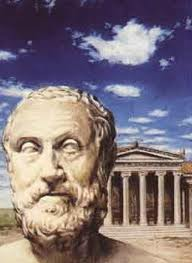
\includegraphics[width=6cm]
  {carneades.png}
\end{center}
\subsection{References}

References should be indexed in some way.

Here they are given  using bibtex to format the entries, which 
in this case are
\cite{ES1}, \cite{ES2}, and \cite{ES3}. 
You \emph{can} use \texttt{bibtex} to prepare references, as here,
or do it by hand if there are very few.

%
\bibliographystyle{plain}
\bibliography{ailp_latex_biblio.bib}
\end{document}

%%% Local Variables:
%%% mode: latex
%%% TeX-master: t
%%% End:
